\documentclass[../main.tex]{subfiles}
\begin{document}
\chapter{Matrices}
\section{Linear Maps}
\begin{definition}[Linear Map]
  Consider two vector spaces $V$ and $W$.
  A \textit{linear map} is a function $T: V \to W$ such that:
  \[
    T(\lambda\vec{x} + \mu\vec{y}) = \lambda T(\vec{x}) + \mu T(\vec{y})
  \]
  for all $\vec{x}, \vec{y} \in V$ and all scalars $\lambda, \mu \in \R \text{ or }\C$ depending on if $V$ and $W$ are real or complex vector spaces.
\end{definition}
\begin{definition}[Domain and Codomain]
  For a linear map $T: V \to W$, $V$ is called the \textit{domain} and $W$ is called the \textit{codomain}.
\end{definition}
\begin{definition}[Image]
  The \textit{image} of a linear map $T$ is:
  \[
    \im T = \{\vec{x}' \in W : \vec{x}' = T(\vec{x}) \text{ for some } \vec{x} \in V\}
  \]
  If $\vec{x}' = T(\vec{x})$ then $\vec{x}'$ is the \textit{image} of $\vec{x}$ under $T$.
\end{definition}
\begin{definition}[Kernel]
  The \textit{kernel} of a linear map $T$ is:
  \[
    \ker T = \{ \vec{x} \in V : T(\vec{x}) = \vec{0}\}
  \]
  If $\vec{x} \in V$ is such that $T(\vec{x}) = \vec{0}$ then we say that $\vec{x}$ belongs to the \textit{kernel} of $T$.
\end{definition}
\begin{proposition}
  For a linear map $T: V \to W$:
  \begin{enumerate}
    \item $\im T$ is a subspace of $W$
    \item $\ker T$ is a subspace of $V$
  \end{enumerate}
\end{proposition}
\begin{proof}
\begin{enumerate}
  \item Let $\vec{u}', \vec{v}' \in \im T$.
    Therefore there exists, $\vec{u}, \vec{v} \in V$ such that $T(\vec{u}) = \vec{u}'$ and $T(\vec{v}) = \vec{v}'$.
    For any scalars $\lambda, \mu$ we have that $\lambda \vec{u} + \mu \vec{v} \in V$ so $T(\lambda \vec{u} + \mu \vec{v}) \in \im T$.
    By linearity, $T(\lambda \vec{u} + \mu \vec{v}) = \lambda \vec{u}' + \mu \vec{v}'$.
    Thus $\lambda \vec{u}' + \mu \vec{v}' \in \im T$ and $\im T \subseteq W$ so $\im T$ is a subspace of $W$.
  \item Let $\vec{u}, \vec{v} \in \ker T$. Therefore $T(\vec{u}) = T(\vec{v}) = \vec{0}$.
    Consider for any scalars $\lambda, \mu$:
    \[
      T(\lambda \vec{u} + \mu \vec{v}) = \lambda T(\vec{u}) + \mu T(\vec{v}) = \vec{0}
    \]
    Thus $\lambda \vec{u} + \mu \vec{v} \in \ker T$ and $\ker T \subseteq V$ so $\ker T$ is a subspace of $V$.
\end{enumerate}
\end{proof}
\begin{definition}[Rank]
  For a linear map $T$ we define the \textit{rank} to be the dimension of the image. That is:
  \[
    \rank T = \dim (\im T)
  \]
\end{definition}
\begin{definition}[Nullity]
  For a linear map $T$ we define the \textit{nullity} to be the dimension of the kernel. That is:
  \[
    \nullity T = \dim (\ker T)
  \]
\end{definition}
\begin{remark}
  If we have a map $T: V \to W$ then $\nullity T = \dim(\ker T) \leq \dim V$ as the kernel is a subspace of $V$ and $\rank T = \dim(\im T) \leq \dim(W)$ as the image is a subspace of $W$.
\end{remark}
\begin{example}
  \begin{enumerate}
    \item \textbf{Zero linear map -} $T: V \to W$ with $\vec{x} \mapsto \vec{0}$.
      Then we have $\im T = \{\vec{0}\}$ and $\ker T = V$.
    \item \textbf{Identity map -} $T: V \to V$ with $\vec{x} \mapsto \vec{x}$.
      Then we have $\im T = V$ and $\ker T = \{\vec{0}\}$.
    \item Consider $T: \R^2 \to \R^2$ and $\vec{x}' = T(\vec{x})$ with:
      \[
        x'_1 = 2x_1 + x_2 \text{ and } x'_2 = x_1 - 3x_2
      \]
      Then:
      \[
        \begin{pmatrix}
        x'_1 \\
        x'_2 \\
        \end{pmatrix} =
        x_1 \begin{pmatrix}
        2 \\
        1 \\
        \end{pmatrix} +
        x_2 \begin{pmatrix}
        1 \\
        -3 \\
        \end{pmatrix}
      \]
      Since $(2, 1)$ and $(1, -3)$ are linearly independent:
      \[
        \im T = \Span\left\{
        \begin{pmatrix}
        2 \\
        1 \\
        \end{pmatrix},
        \begin{pmatrix}
        1 \\
        -3 \\
        \end{pmatrix}
        \right\} =
        \left\{
        \lambda\begin{pmatrix}
        2 \\
        1 \\
        \end{pmatrix} +
        \mu\begin{pmatrix}
        1 \\
        -3 \\
        \end{pmatrix},\ \lambda, \mu \in \
        \right\}
      \]
      Furthermore, $2x_1 + x_2 = 0$ and $x_1 - 3x_2 = 0 \implies x_1 = x_2 = 0$ so:
      \[
        \ker T = \left\{\begin{pmatrix}
        0 \\
        0 \\
        \end{pmatrix}\right\}
      \]
  \end{enumerate}
\end{example}
\subsubsection{Linear Combinations}
Consider linear maps $T, S: V \to W$.
Then $\alpha T + \beta S: V \to W$ is also a linear map defined by:
\[
  (\alpha T + \beta S)(\vec{x}) = \alpha T(\vec{x}) + \beta S(\vec{x})
\]
for $\alpha, \beta \in \R \text{ or } \C$.
\subsubsection{Composition}
Take linear maps $T: V \to W$ and $S: U \to V$.
Then $U \xrightarrow{S} V \xrightarrow{T} W$ so $T \circ S: U \to W$.
This composition is also a linear map, defined by:
\[
  (T \circ S)(\vec{x}) = T(S(\vec{x}))
\]
\begin{theorem}[Rank-nullity Theore]
  For a linear map $T: V \to W$ then:
  \[
    \label{rankNullity}
    \rank T + \nullity T = \dim V
  \]
\end{theorem}
\begin{proof}
\nonexaminable
Let $n$ be $\dim V$ and $m$ be $\nullity T$.
\[
  \nullity T = \dim (\ker T) \leq \dim V \iff m \leq n
\]
So we only need to consider $m \leq n$.
\begin{proofcases}
  \begin{case}{$m = n$}
    Then $\dim(\ker T) = \dim V$ and since $\ker T$ is a subspace of $V$, we must have $\ker T = V$.
    Therefore $\im T = \{\vec{0}\}$.
    So $\rank T + \nullity T = \dim(\im T) + \dim(\ker T) =0 + n = n$.
  \end{case}
  \begin{case}{$m < n$}
    Let $\{\vec{e}_1, \ldots, \vec{e}_m\}$ be a basis of the kernel of T.
    So $T(\vec{e}_i) = \vec{0}$ for all $i = 1, \ldots, m$.
    We can now extend $\{\vec{e}_1, \ldots, \vec{e}_m\}$ to form a basis of $V$.
    Since $\dim V = n$ the basis must have $n$ elements so:
    \[
      \{\vec{e}_1, \ldots, \vec{e}_m, \vec{e}_{m+1}, \ldots, \vec{e}_n\}
    \]
    We now need to show that $B = \{T(\vec{e}_{m + 1}), \ldots, T(\vec{e}_n)\}$ is a basis of $\im T$.
    \begin{enumerate}
      \item
      To show that $B$ spans $\im T$, take an element $\vec{y} \in \im T$.
      Then by definition, there exists $\vec{x} \in V$ such that $T(\vec{x}) = \vec{y}$.
      Since $\vec{x} \in V$, we can write:
      \[
        \vec{x} = \alpha_1 \vec{e}_1 + \cdots + \alpha_n \vec{e}_n
      \]
      Applying $T$ to this yields:
      \begin{align*}
        \vec{y} = T(\vec{x}) &= T(\alpha_1 \vec{e}_1 + \cdots + \alpha_n \vec{e}_n) \\
                             &= \alpha_1 T(\vec{e}_1) + \cdots \alpha_n T(\vec{e}_n) \\
                             &= \alpha_{m + 1} T(\vec{e}_{m + 1}) + \cdots + \alpha_n T(\vec{e}_n)
      \end{align*}
      Therefore, any element in $\im T$ can be written as a linear combination of vectors from $B$, thus $B$ spans $\im T$.
      \item
      To show that $B$ is linearly independent, consider:
      \[
        \alpha_{m + 1} T(\vec{e}_{m+1}) + \cdots + \alpha_n T(\vec{e}_n) = \vec{0}
      \]
      We now need to show that all of the coefficients are 0.
      By linearity we can write this as:
      \[
        T(\underbrace{\alpha_{m + 1}\vec{e}_{m + 1} + \cdots + \alpha_n \vec{e}_n}_{\vec{x}}) = \vec{0}
      \]
      So $\vec{x} \in \ker T$ and the basis of $\ker T$ is $\{\vec{e}_1, \ldots, \vec{e}_n\}$.
      Therefore there exists $\alpha_1, \cdots \alpha_m$ such that:
      \[
        \vec{x} = \alpha_1 \vec{e}_1 + \cdots + \alpha_m \vec{e}_m
      \]
      We can now equate our two expressions for $\vec{x}$ to get:
      \[
        \alpha_1 \vec{e}_1 + \cdots \alpha_m \vec{e}_m - \alpha_{m + 1}\vec{e}_{m + 1} - \cdots - \alpha_n \vec{e}_n = \vec{0}
      \]
      However $\{\vec{e}_1, \ldots, \vec{e}_m, \vec{e}_{m + 1}, \ldots, \vec{e}_n\}$ is a basis of $V$.
      Since the elements of a basis must be linearly independent, all the coefficients must be 0.
      Thus:
      \[
        \alpha_1 = \cdots = \alpha_m = \alpha_{m + 1} = \cdots = \alpha_n = 0
      \]
      So $B$ is linearly independent.
    \end{enumerate}
    Therefore $B$ is a basis of $\im T$ and so $\rank T = \dim(\im T) = n - m$ as $B$ has $n - m$ elements.
    Thus:
    \[
      \rank T + \nullity T = n - m + m = n = \dim V
    \]
  \end{case}
\end{proofcases}
\end{proof}
\begin{example}
  \begin{enumerate}
    \item For the zero map, $\nullity T = \dim V$ and $\rank T = 0$ so $\nullity T + \rank T = \dim V$.
    \item For the identity map, $\rank T = \dim V$ and $\nullity T = 0$ so $\nullity T + \rank T = \dim V$.
  \end{enumerate}
\end{example}
\section{Matrices as Linear Maps}
Let $M$ be a matrix with entries $M_{i j} \in \R$, where $i$ labels rows and $j$ labels columns.
Then the map defined by $T: \R^{n} \to \R^{n}$, $T(\vec{x}) = \vec{x}' = M\vec{x}$ for $\vec{x}, \vec{x}' \in \R^{n}$ with $x'_i = M_{i j}x_j$, is a linear map.
\begin{example}
  Given $n = 2$:
  \[
    M = \begin{pmatrix}
    M_{1 1} & M_{1 2} \\
    M_{2 1} & M_{2 2} \\
    \end{pmatrix}
  \]
  so we have:
  \[
    \begin{pmatrix}
    x'_1 \\
    x'_2 \\
    \end{pmatrix}
    =
    \begin{pmatrix}
    M_{1 1} & M_{1 2} \\
    M_{2 1} & M_{2 2} \\
    \end{pmatrix}
    \begin{pmatrix}
    x_1 \\
    x_2 \\
    \end{pmatrix}
    =
    \begin{pmatrix}
    M_{1 1}x_1 + M_{1 2}x_2 \\
    M_{2 1}x_1 + M_{2 2}x_2 \\
    \end{pmatrix}
  \]
\end{example}
We can also consider the rows and columns of $M$ as vectors in $\R^{n}$.
We can denote the rows as $\vec{R}_i \in \R^{n}$ and the columns as $\vec{C}_i \in \R^{n}$:
\[
  M = \begin{pmatrix}
  \leftarrow \vec{R}_1 \rightarrow \\
  \cdots \\
  \leftarrow \vec{R}_n \rightarrow
  \end{pmatrix}
  =
  \begin{pmatrix}
  \uparrow & & \uparrow  \\
  \vec{C}_1 & \cdots & \vec{C}_n  \\
  \downarrow &  & \downarrow \\
  \end{pmatrix}
\]
The components are then related in the following form:
\[
  M_{i j} = (\vec{C}_j)_i = (\vec{R}_i)_j
\]
If $\{\vec{e}_1, \ldots, \vec{e}_n\}$ is the standard basis of $\R^{n}$:
\[
  \vec{e}_i \mapsto \vec{e}_i' = T(\vec{e}_i) = M\vec{e}_i = \vec{C}_i
\]
That is, multiplying a matrix by the $i$-th element of the standard basis extracts the $i$-th column.
\[
  \begin{pmatrix}
  M_{1 1} & \cdots & M_{1 n} \\
  \vdots & \ddots & \vdots \\
  M_{n 1} & \cdots & M_{m n} \\
  \end{pmatrix}
  \vec{e}_i = \vec{C}_i
\]
Since $T$ is a linear map for any $\vec{x} \in \R^{n}$:
\[
  \vec{x} = \sum_{i} x_i \vec{e}_i \mapsto T\left(\sum_{i} x_i \vec{e}_i \right) = \sum_{i} x_i \vec{C}_i
\]
Thus $\vec{x} \mapsto x_i \vec{C}_i$.
This means the image of $\vec{x}$ under $T$ a linear combination of the columns of the matrix.
Therefore, $\im T = \im M = \Span\{\vec{C}_1, \ldots, \vec{C}_n\}$.

We can also determine the kernel of $T$ using its matrix representation.
Consider an element of the image, $\vec{x}'$, of $\vec{x}$ under $T$:
\[
  x_i' = M_{i j}x_j = (\vec{R}_i)_j x_j = \vec{R}_i \cdot \vec{x}
\]
so
\[
  \vec{x}' = \begin{pmatrix}
  x_i' \\
  \vdots \\
  x_n' \\
  \end{pmatrix}
  =
  \begin{pmatrix}
  \vec{R}_i \cdot x \\
  \vdots \\
  \vec{R}_n \cdot x \\
  \end{pmatrix}
\]
If $\vec{x} \in \ker T$ then $\vec{x}' = \vec{0}$ so $\vec{R}_1 \cdot \vec{x} = \cdots = \vec{R}_n \cdot \vec{x} = 0$.
Therefore the kernel of $T$ is all vectors that are orthogonal to all rows of the matrix:
\[
  \ker T = \ker M = \{\vec{x} \in \R^{n}: \vec{R}_i \cdot \vec{x} = \vec{0},\ \forall i = 1, \ldots n\}
\]
This is a subspace of $\R^{n}$ as a linear combination of such vectors would also satisfy the above property and therefore would also be in the subspace.
\begin{remark}[Summary]
  \begin{itemize}
    \item $\im M$ is the span of the columns of $M$.
    \item $\ker M$ is the subspace orthogonal to all rows of $M$.
  \end{itemize}
\end{remark}
\begin{example}
  \begin{enumerate}
    \item For $T: \R^{n} \to \R^{n}$, the zero map has representation $\vec{x}' = O\vec{x}$ where $O_{ij} = 0\ \forall i, j$.
      This matrix is called the \textit{zero matrix}.
    \item For $T: \R^{n} \to \R^{n}$, the identity map has representation $\vec{x}' = I\vec{x}$ where $I_{i j} = \delta_{i j}$.
      This matrix is called the \textit{identity matrix}.
    \item For $T: \R^3 \to \R^3$, $\vec{x}' = M \vec{x}$ given by:
      \begin{align*}
        x_1' &= 3x_1 + x_2 + 5x_3 \\
        x_2' &= -x_1 + 2x_3 \\
        x_3' &= 2x_1 + x_2 + 3x_3
      \end{align*}
      This can be converted into matrix form:
      \[
        M = \begin{pmatrix}
        3 & 1 & 5 \\
        -1 & 0 & -2 \\
        2 & 1 & 3 \\
        \end{pmatrix}
      \]
      Since $\im(T)$ is the span of the columns:
      \[
        \im T = \Span\{\vec{C}_1, \vec{C}_2, \vec{C}_3\} = \Span\{\vec{C}_1, \vec{C}_2\}
      \]
      As $\vec{C}_3 = 2\vec{C}_1 - \vec{C}_2$.
      Since $\vec{C}_1, \vec{C}_2$ are linearly independent, $\rank T = \dim(\im T) = 2$.
      From \cref{rankNullity} (rank nullity theorem), we expect $\nullity T = 1$.

      To find $\ker T$ we need to find the subspace orthogonal to all rows.
      \[
        \vec{R}_2 \times \vec{R}_3 = \begin{vmatrix}
        \uvec{i} & \uvec{j} & \uvec{k} \\
        -1 & 0 & -2 \\
        2 & 1 & 3 \\
        \end{vmatrix} =
        \begin{pmatrix}
        2 \\
        -1 \\
        -1 \\
        \end{pmatrix}
      \]
      This is also orthogonal to $\vec{R}_1$ thus:
      \[
        \ker T = \ker M = \Span\left\{
        \begin{pmatrix}
        2 \\
        -1 \\
        -1 \\
        \end{pmatrix}\right\}
      \]
      Since this has dimension 1, $\nullity T = 1$, as expected.
  \end{enumerate}
\end{example}
\section{Geometric Examples\texorpdfstring{ in $\R^2$ and $\R^3$}{}}
\subsection{Examples in \texorpdfstring{$\R^2$}{2D}}
\subsubsection{Rotations}
Consider $\theta$ such that $-\pi < \theta \leq \pi$, then a rotation by angle $\theta$ anticlockwise in $\R^2$ can be represented by:
\[
  \Rot(\theta) = \begin{pmatrix}
  \cos \theta & -\sin \theta \\
  \sin \theta & \cos \theta \\
  \end{pmatrix}
\]
Note that $\det(\Rot(\theta)) = \cos^2 \theta + \sin^2 \theta = 1$.
\begin{center}
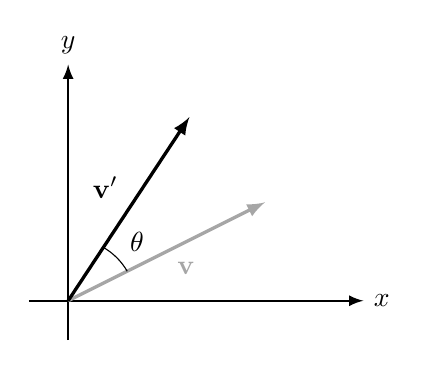
\begin{tikzpicture}[scale=2.5,>=latex]
\draw[->, thick] (-0.2,0) -- (1.5,0) node[right] {$x$};
\draw[->, thick] (0,-0.2) -- (0,1.2) node[above] {$y$};

\coordinate (A) at (1, 0.5);
\coordinate (B) at ({cos(30)*1 - sin(30)*0.5}, {sin(30)*1 + cos(30)*0.5});

\draw[->, very thick, gray!70] (0,0) -- (A) node[midway, below right] {$\mathbf{v}$};

\draw[->, very thick, black] (0,0) -- (B) node[midway, above left] {$\mathbf{v}'$};

\draw[-, black] (0.3,0.15) arc[start angle=30, end angle=60, radius=0.33];
\node at (0.35,0.3) {$\theta$};
\end{tikzpicture}
\end{center}
\subsubsection{Reflections}
Consider $\theta$ such that $-\pi < \theta \leq \pi$, then reflection in the line with angle $\frac{\theta}{2}$ anticlockwise from the $x$-axis (i.e. $y = x\tan(\theta/2)$) in $\R^2$ is represented by:
\[
  \Reflect(\theta) = \begin{pmatrix}
  \cos \theta & \sin \theta \\
  \sin \theta & -\cos \theta \\
  \end{pmatrix}
\]
Note that $\det(\Reflect(\theta)) = -\cos^2 \theta - \sin^2 \theta = -1$.
\begin{center}
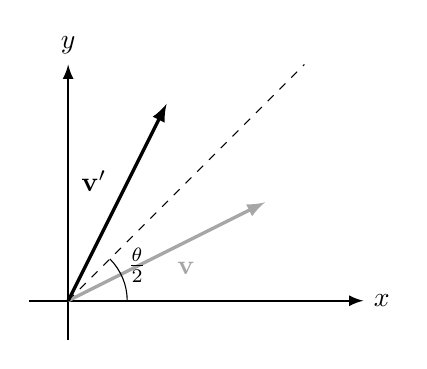
\begin{tikzpicture}[scale=2.5,>=latex]
\draw[->, thick] (-0.2,0) -- (1.5,0) node[right] {$x$};
\draw[->, thick] (0,-0.2) -- (0,1.2) node[above] {$y$};

\coordinate (A) at (1, 0.5);
\coordinate (B) at (0.5, 1);

\draw [black, dashed] (0, 0) -- (1.2, 1.2);
\draw[->, very thick, gray!70] (0,0) -- (A) node[midway, below right] {$\mathbf{v}$};

\draw[->, very thick, black] (0,0) -- (B) node[midway, above left] {$\mathbf{v}'$};

\draw[-, black] (0.3,0) arc[start angle=0, end angle=45, radius=0.3];
\node at (0.35,0.18) {$\frac{\theta}{2}$};
\end{tikzpicture}
\end{center}
\subsubsection{Properties}
\begin{enumerate}
  \item $\Rot(\theta)\Rot(\phi) = \Rot(\theta + \phi)$
  \item $\Reflect(\theta)\Reflect(\phi) = \Rot(\theta - \phi)$
  \item $\Rot(\theta)\Reflect(\phi) = \Reflect(\phi + \theta)$
  \item $\Reflect(\theta)\Rot(\theta) = \Reflect(\phi - \theta)$
\end{enumerate}
\subsection{Examples in \texorpdfstring{$\R^3$}{3D}}
\subsubsection{Rotation along a basis}
Rotation of angle $\theta$ with axis $\vec{e}_1, \vec{e}_2, \vec{e}_3$:
\begin{align*}
  \Rot_{\vec{e}_1}(\theta) &= \begin{pmatrix}
  1 & 0 & 0 \\
  0 & \cos \theta & -\sin \theta \\
  0 & \sin \theta & \cos \theta \\
  \end{pmatrix} \\
  \Rot_{\vec{e}_2}(\theta) &= \begin{pmatrix}
  \cos \theta & 0 & \sin \theta \\
  0 & 1 & 0 \\
  - \sin \theta & 0 & \cos \theta \\
  \end{pmatrix} \\
  \Rot_{\vec{e}_3}(\theta) &= \begin{pmatrix}
  \cos \theta & -\sin \theta & 0 \\
  \sin \theta & \cos \theta & 0 \\
  0 & 0 & 1 \\
  \end{pmatrix}
\end{align*}
\begin{remark}[Warning]
  These look like they all have the same format, however, for $\vec{e}_2$, the negative is on the other $\sin \theta$.
\end{remark}
\subsubsection{Rotation about a unit vector}
Consider a rotation of $\theta$ about a unit vector $\vec{n}$.
For $x \in \R^{3}$
\[
  \vec{x}' = R\vec{x},\ \vec{x}_i' = R_{i j}x_j
\]
We can write:
\[
  \vec{x}' = (\cos \theta)\vec{x} + (1 - \cos \theta)(\vec{n} \cdot \vec{x})\vec{n} + (\sin \theta)(\vec{n} \times \vec{x})
\]
Or equivalently:
\[
  R_{i j} = \delta_{i j}\cos\theta + (1 - \cos \theta)n_in_j - (\sin \theta)\levi_{i j k}n_k
\]
We could express this in matrix form, however it would be quite messy.

To show why this is a rotation of $\vec{x}$ about $\vec{n}$, we can first split $\vec{x}$ into a component parallel to $\vec{n}$ and a component perpendicular to $\vec{n}$:
\[
  \vec{x} = \vec{x}_{\parallel} + \vec{x}_{\perp}
\]
where $\vec{x}_{\parallel} = (\vec{x} \cdot \vec{n})\vec{n}$ and $\vec{x}_{\perp}$ such that $\vec{n} \cdot \vec{x}_{\perp} = 0$.

After applying $R$, $\vec{x}_{\parallel}$ is unchanged as it is parallel to the axis of rotation, so $\vec{x}_{\parallel}' = \vec{x}_{\parallel}$.
To find the image of $\vec{x}_{\perp}$, consider the plane orthogonal to $\vec{n}$ and vector $\vec{n} \times \vec{x}$:
\begin{center}
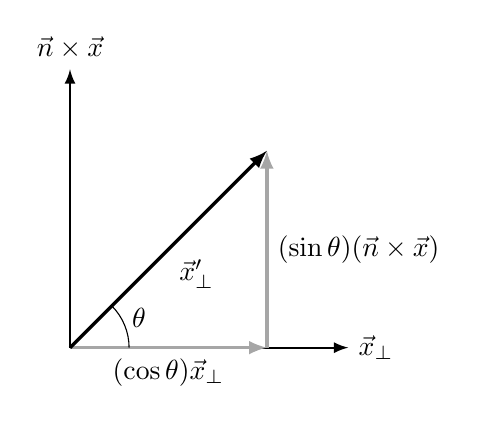
\begin{tikzpicture}[scale=2.5,>=latex]
\draw[->, thick] (0,0) -- (1.414,0) node[right] {$\vec{x}_{\perp}$};
\draw[->, thick] (0,0) -- (0,1.414) node[above] {$\vec{n} \times \vec{x}$};

\draw[->, very thick, gray!70] (1, 0) -- (1, 1) node[midway, right, black] {$(\sin \theta)(\vec{n} \times \vec{x})$};
\draw[->, very thick, gray!70] (0, 0) -- (1, 0) node[midway, below, black] {$(\cos \theta)\vec{x}_{\perp}$};
\draw[->, very thick] (0,0) -- (1,1) node[midway, below right] {$\vec{x}_{\perp}'$};

\draw[black] (0.3,0) arc[start angle=0, end angle=45, radius=0.3];
\node at (0.35,0.15) {$\theta$};
\end{tikzpicture}
\end{center}
We get $(\sin \theta)(\vec{n} \times \vec{x})$ as $|\vec{x}_{\perp}| = |\vec{n} \times \vec{x}|$ (consider the projection of $\vec{x}$ onto the plane orthogonal to $\vec{n}$) and $\vec{n} \times \vec{x}$ is in the correct direction.

Therefore:
\[
  \vec{x}_{\perp}' = (\cos \theta)\vec{x}_{\perp} + (\sin \theta)(\vec{n} \times \vec{x})
\]
Since $\vec{x} = \vec{x}_{\parallel} + \vec{x}_{\perp} \implies \vec{x}_{\perp} = \vec{x} - (\vec{x} \cdot \vec{n})\vec{n}$.
So we can write:
\[
  \vec{x}_{\perp}' = (\cos \theta)\vec{x} - (\cos \theta)(\vec{x} \cdot \vec{n})\vec{n} + (\sin \theta)(\vec{n} \times \vec{x})
\]
As it is a linear map, the image of $\vec{x}$ is just the sum of the images of its components so:
\[
  \vec{x}' = \vec{x}_{\parallel}' + \vec{x}_{\perp}' = (\cos \theta)\vec{x} + (1 - \cos\theta)(\vec{x} \cdot \vec{n})\vec{n} + (\sin \theta)(\vec{n} \times \vec{x})
\]
\subsubsection{Reflections}
Reflections in a plane passing through the origin with unit normal vector $\vec{n}$ are represented by:
\[
  \vec{x}' = H\vec{x} = \vec{x} - 2(\vec{x} \cdot \vec{n})\vec{n}
\]
Note that $(\vec{x} \cdot \vec{n})\vec{n}$ is the vector projection of $\vec{x}$ onto $\vec{n}$.
This can be seen in the following diagram:
\begin{center}
\begin{tikzpicture}[scale=2.5,>=latex]
\draw[thick, dotted] (-1.5,0) -- (1.5,0) node[right] {$\text{Plane}$};
\draw[->, thick] (0,0) -- (0,1) node[above] {$\vec{n}$};

\draw[dashed, gray!70] (1, 1) -- (1, -1);
\draw[->, thick] (1, 0) -- (1, 1) node[midway, right] {$(\vec{x} \cdot \vec{n})\vec{n}$};
\draw[->, very thick] (0,0) -- (1,1) node[midway, below right] {$\vec{x}$};
\draw[->, very thick] (0,0) -- (1,-1) node[midway, below left] {$\vec{x}'$};

\node[below left] at (0, 0) {$O$};
\end{tikzpicture}
\end{center}
This has matrix representation given by:
\[
  \vec{x}_i' = H_{i j}x_j,\ H_{i j} = \delta_{i j} - 2n_in_j
\]
So:
\[
  H = \begin{pmatrix}
  1-2n^{2}_{1} & -2n_1n_2 & -2n_1n_3 \\
  -2n_1n_2 & 1-2n^{2}_{2} & -2n_2n_3 \\
  -2n_1n_3 & -2n_2n_3 & 1-2n^{2}_{3} \\
  \end{pmatrix}
\]
\end{document}
